%%%%%%%%%%%%%%%%%%%%%%%%%%%%%%%%%%%%%%%%%%%%
In this chapter we study the problem of Sinkless Orientation. The work was done as part of a joint work with Sebastian Brandt, Juho Hirvonen, Barbara Keller, Tuomo Lempi{\"{a}}inen, Joel Rybicki, Jukka Suomela and Jara Uitto $\cite{BFHKLRSU16}$. The work gives a new type of lower bound in the LOCAL model, and gave a $\Omega(\log\log n)$ lower bound on the distributed Lova'sz Local Lemma, improving the previous lower bound of $\Omega(\log^*n)$ by \cite{KMPHH14}. A followup work by  $\cite{CKP16}$ showed using similar techniques the first exponential separation between randomized and deterministic round complexity in the LOCAL model, solving an important open problem in distributed computing. This section details the reduction to the local lemma, and a deterministic $O(\log n)$ solution for this problem, and shows how to solve variants of the problem such as sinkless sourceless orientation.  We further show that the algorithm can be adapted to the CONGEST model, in which each edge has a restricted bandwidth per round of communication. This result is new and unpublished prior to this thesis. We note that the $O(\log n)$ deterministic algorithm in the LOCAL model in section \ref{AlgSection} is nearly identical to an algorithm in \cite{GS2017} and was developed independently and in parallel of it.

\section{Preliminaries}

\paragraph{The Distributed LOCAL Setting}
In this model we have $n$ processors, who are connected in a communication network graph $G$. The processors only know their neighbors and are oblivious to the rest of the network. The processors may communicate with each other in synchronous rounds, and in each round each processors may send a message (of unlimited size) to each of its neighbors, and it may also output a value of its choice, terminating its role in the network. It is further assumed that each processor has unlimited computational power. 

Denote the graph output as a vector of size $n$,  such that in the $i$'th coordinate contains the output of vertex $i$. A local distributed problem $P$ is defined as a set of valid graph outputs per communication graph $G$. The goal of the processors is to output so that the output of the graph would be valid. The round complexity of a deterministic protocol is defined as the number of rounds it takes for all the processors running the protocol to terminate. For randomized algorithms this is defined as the worst case round over the coins of the processors. The round complexity of $P$ defied as the minimal round complexity of a protocol solving $P$ with probability at least $\frac{2}{3}$.

\paragraph{Notations}
Denote $\delta$ as the minimal degree in $G$, and denote $dist(v,u)$ as the distance between $u$ and $v$ in the communication graph $G$. For a set of vertices $A$, let $dist(A,u) = \min_{v \in A}{dist(v,u)}$.

\section{Sinkless Orientation}
The sinkless orientation problem is defined as follows:
\begin{problem} Given a graph $G=(V,E)$ with minimal degree $\delta \geq 3$, output an orientation for each edge such that the minimal out degree of each vertex is at least $1$. 
\end{problem}

In order for this problem to be well defined, there should exist a sinkless orientation for any such graph. We show this is the case in the following claim, which also gives us a better understanding of the sinkless orientation's nature.

\begin{claim}
	Given a graph $G=(V,E)$ with minimal degree $\delta \geq 2$, there exists a sinkless orientation.
\end{claim}
\begin{proof}
	Fix a connected component $G_1$ in $G$. Since the degree of each vertex is at least $2$, there exists a cycle in $G_1$. Fix such a cycle $C$, and consider an orientation of its edges such that the cycle is oriented in one of its two directions. For each vertex not in the cycle we do a "reverse BFS" from the cycle to the rest of the graph, orienting the edges inwards. Formally let $Level_i(C) = \{v|dist(C,v) = i\}$ be a partition to BFS layers from the cycle. For each vertex in $Level_i$ there exists a neighbor in $Level_{i-1}$. Orienting each vertex towards its parent, each vertex in level $\geq 1$ has an outgoing edge, while vertices on $Level_0$ are on the cycle and therefore have an outgoing edge. By orienting the rest of the edges arbitrarily, an sinkless orientation is obtained.
\end{proof}


\begin{claim}
	Fix an oriented graph edges as $\vec{E}$ and the associated directed graph $\vec{G}$. $\vec{G}$ is a sinkless orientation if and only if every $v \in \vec{G}$ has a path to a cycle in $\vec{G}$.
\end{claim}
\begin{proof}
	If $v$ has a directed path to a cycle, trivially $v$ has an outwards edge. Assume $\vec{G}$ has no sinks, and let $v_1$ be a vertex in $G$. Consider a path $v_1v_2v_3...v_{n+1}$, which is obtained by following an arbitrary outgoing edge from $v_i$ in the $i$'th step. Such an edge always exists since all vertices have an outwards edge. Since the path is of length $n+1$, the path contains a cycle.
\end{proof}

The original paper \cite{BFHKLRSU16} shows a $\Omega(\log\log{n})$ lower bound on the the Symmetric Distributed Algorithmic Local Lemma problem $\cite{BFHKLRSU16}$, using a $\Omega(\log\log{n})$ lower bound  on randomized sinkless orientation on developed in the paper. For this purpose, a reduction from LLL to 3-regular 3-edge-colored is shown in section \ref{sec:rand_lovasz}.

\begin{problem}
	Given a d-regular graph $G$, $d \geq 3$, output a sinkless orientation on $G$.
\end{problem}

A reduction for the case $d \geq 4$ is immediate. The interesting case is $d=3$, which is solved by a combinatorial reduction to $d=4$. This shows that an LLL instance is hard even for dependency $d=3$. 





\section{An $O(\log{n})$ Deterministic Algorithm Problem in the LOCAL model} \label{AlgSection}
\subsection{Problem Definition}
This section describes an algorithm to solve the sinkless orientation problem under the LOCAL model in $O(\log{n})$ rounds. This was developed independently and in parallel to a nearly identical algorithm in \cite{GS2017}. 

The key observation for the algorithm is that for $G$ such that $\delta \geq 3$ any vertex in $G$ is of distance at most $\log{n}$ from a cycle of length at most $\log{n}$.  The main idea of the algorithm is for each vertex to find such a cycle close to it, and to attempt to direct itself to the cycle, and direct the cycle in one of its two orientations. Of course, as all vertices attempt this simultaneously there could be contradicting manners in which an edge can be ordered to be directed. For this, we introduce order priorities. In the algorithm, when a vertex $v$ sends an order to direct a (distant) edge, it assigns the order a priority $k=v.id$. At the end of the algorithm, an edge will determine its final orientation by the orientation order with the maximal priority it received during the course of the algorithm.


\subsection{Algorithm Description}
\begin{algorithm}[H]\label{SinklessLocal}\small
\caption{\small SinklessLocal($v,Neigbors,Id$)}
\begin{itemize}
\item\begin{bf}For\end{bf} {$i=1,...,\log{n}$}:
\begin{itemize}
\item Gathers neighbors of distance $i$.   
\end{itemize}
\item Let $c$ be the lexicographically smallest observed cycle in the $\log{n}$ neighborhood, and let $p$ be the lexicographically smallest shortest path from $v$ to $c$.
\item With order priority $=v.id$, Send direction orders to Direct $p$ in the direction of $c$, and to direct the cycle $c$ in the following direction: Let $a$ be the vertex with the highest Id in the $c$, and let $b$ be the neighbor in $c$ with the larger Id., and direct it in the direction so that $a \rightarrow b$.
\item After $3\log{n}$ rounds, orient each unoriented edge towards the higher Id vertex, and terminate.
\end{itemize}
\end{algorithm}


\begin{lemma}
	\label{lem:near_cycle}
If $\delta \geq 3$, Then each vertex there exists a cycle of size $\log{n}$ is at distance at most  from a cycle of length at most $\log{n}$ .
\end{lemma}
\begin{proof}
Assume by contradiction that there exists $v \in V$ for which that does not hold, meaning that in the $\log{n}$ neighborhood of $v$ is a tree. Consider its $\log{n}$ neighborhood, and denote $Level_i(v) = \{u|dist(v,u) = i\}$ the BFS layers of the vertex $v$. Since there are no cycles, the $\log{n}$ neighborhood of $v$ is a tree, and since the degree of each vertex is at least $3$, $|level_{i+1}| \geq 2 \cdot |level_i|$. The $\log{n}$ neighborhood has $1+2^{\log{n}} = n+1 > n$ vertices, contradiction, since there are only $n$ vertices in the graph.
\end{proof}

\begin{corollary}
$SinklessLocal$ terminates after $O(\log{n})$ rounds. At the end of the algorithm each vertex has an outgoing edge.
\end{corollary}
\begin{proof}
The protocol explicitly terminates after $3\log{n}$ rounds. Note that both the neighbor gathering phase and the direction order phase complete successfully as from the previous lemma, the neighborhood gathering phase terminates after $\log{n}$ rounds, since there exists a cycle of size $\log{n}$ in its $\log{n}$ neighborhood. This also means that the directing phase terminates after $\log{n}$ rounds.  Let $v \in V$, and let $k$ be the maximum priority $v$ encounters during the algorithm. From the definition of orientation priorities, there exists some vertex $u$ with $id=k$ that sent the orientation order to $e$. Since $u$ sent orientation orders to a cycle and the path to it, $u$ also sent an orientation order to an edge $e$ leaving $v$ with priority also $k$. and since $k$ is the maximum priority seen by $v$ and the fact that id's are unique, then this order has the highest priority on $e$, and thus at the end of the algorithm $e$ is oriented outwards from $v$.
\end{proof}
\begin{figure}[h]
	\centering
	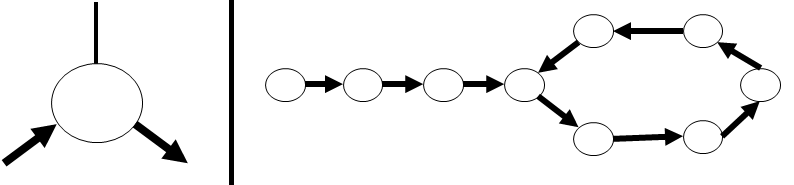
\includegraphics[width=0.5\textheight]{img/sinklessProof}
	\caption{As an orientation order consists of a directed path connected to a cycle (where each vertex has out-degree $> 1$), each order encountered by a vertex has an order to orient one of its an edges outwards from it, so such an edge associated with the highest id encountered is oriented outwards at the end of the algorithm.}
\end{figure}

\begin{theorem}
$SinklessLocal$ is a procedure that outputs a sinkless orientation and terminates after $O(\log{n})$ rounds.
\end{theorem}

%%%%%%%%%%%%%%%%%%%%%%%%%%%%%%%%%%%%%%%%%%%%
\section{Randomized Sinkless algorithm using Algorithmic local Lemma}
\label{sec:rand_lovasz}
This section aims to reduce the sinkless orientation problem for $d$ regular graph to the Distributed Lovaz Algorithmic local Lemma (LLL) with variable dependency $d$ (To be defined later). The first result gives a reduction from LLL to any $d$ using an assumption of $d$-edge coloring, which is sufficient for the original lower bound purposes, and the second result shows how to lift the need of $d$-edge coloring using maximal matching, and extending the results to many related problems, such as sinkless sourceless orientation.

\subsection{Distributed Algorithms for the Lovasz Local Lemma }
The setting of the Symmetric Algorithmic Lovasz Local Lemma by Moser and Tardos \cite{MoserT10} is the following: 
\begin{problem}[Moser and Tardos]
Let $P$ be a finite set of mutually independent random variables in a probability space. Let $\mathcal{A}$ be an set of events, $p \in [0,1]$ such that  for any event $A \in \mathcal{A}$, $Pr(A) \leq p$ , and each event in $\mathcal{A}$ share variables with at most $d$ other events. Given that $ep(d+1) < 1$, Find an assignment for all variables such that no event in $\mathcal{A}$ occurs.
\end{problem}

the dependency graph $G_{\mathcal{A}}$, is defined as a graph where each $A \in \mathcal{A}$ is a vertex, and two vertices have an edge if they share common variables (are Dependant). In the distributed model we assume that our communication graph is the dependency graph, and our goal is for each vertex to output a value of its variables such that the problem no $A \in \mathcal{A}$ occurs.

In $\cite{KMPHH14}$, two distributed LLL algorithms were developed for the LOCAL model, with slightly different dependence assumptions. Given  $ep(d+1) < 1$, there is an algorithm  for solving a LLL instance in running in $O(log^2(d) \cdot \log{n})$ rounds, and given $epd^2 < 1$ it can be done in $O(\log{n})$ rounds. 

\begin{definition}
Given a d-regular graph $G=(V,E)$, define a random variable for each edge to be its direction, and for each $v \in V$ define a bad event $A_v=$"$v$ is a sink" ($out\text{-}deg(v) = 0$). Let $G_{Sink}$ be the dependency graph of these bad events and probability space. 
\end{definition} 
\begin{lemma}
	\label{lem:rand_sink_dep_graph}
The following observations hold for $G_{Sink}$:
\begin{compactenum}
\item $A_v$  shares variables with  $A_u$ if and only if $(u,v) \in E$.
\item The dependency graph $G_{Sink}$ is isomorphic to $G$, and  $\phi(v) =A_v$ is an isomorphism function.
\item $Pr(A_v) = \frac{1}{2^d}$	
\end{compactenum}
\end{lemma}
\begin{proof}
For (1), since the independent variables are the edge directions, if $u,v$ are not neighbors, then "$u$ is a sink" and "$v$ is a sink" do not share a common variable. In the other direction if $u,v$ are neighbors and $u$ is a sink, then the edge between $u$ and $v$ must be directed $(v,u)$, meaning $v$ isn't a sink, thus $A_v$ and $A_u$ are dependent. Note that (2) follows immediately from the first claim and the definition of the dependency graph. 

Claim (3) holds since $G$ is a d-regular graph, so the probability of a bad event $A_v$ is $\frac{1}{2^d}$, as the edge directions are chosen i.i.d uniformly.
\end{proof}


\subsection{$O(\log{n})$ Algorithm on d-regular graphs with $d > 3$}
This subsection gives the description of the algorithm for $d > 3$. This follows directly by applying the LLL algorithm.

\begin{lemma}
Given a 4-regular graph, a sinkless orientation can be found in $O(\log{n})$ rounds using the distributed algorithmic local lemma.
\end{lemma}
\begin{proof}
For an i.i.d random choice of edge directions,  it holds that for any $A_v$,  $ P(A_v) = \frac{1}{16}$, meaning $ep(d+1) = \frac{e \cdot 5}{16} < 1$, therefore by the distributed algorithmic local lemma it can be solved in $O(\log{n})$ rounds.  
\end{proof}

\begin{corollary}
Given a d-regular graph, $d > 3$, a sinkless orientation can be found in $O(\log{n})$ rounds using the distributed algorithmic local lemma.
\end{corollary}
\begin{proof}
	For $4 \leq d \leq 8$ the algorithm in $\cite{KMPHH14}$ terminates after $O(log^2(d) \cdot \log{n}) = O(\log{n})$ rounds w.h.p, and gives direction assignments to each edge. For $d > 8$ the stronger $epd^2 < 1$ holds so using the second LLL algorithm in$\cite{KMPHH14}$, an LLL can be obtained in $O(\log{n})$ rounds.
\end{proof}

\subsection{$O(\log{n})$ Algorithm on 3-regular graphs}
Unfortunately, for the 3-regular case, the Local Lemma is not directly applicable since $ep(d+1) > 1$. We show a reduction to the 4-regular case. 

The key observation is that two 3-degree adjacent vertices act together like a single 4-degree vertex: if we contract the two adjacent vertices into one by their common edge, the new vertex has 4 edges, and if the graph was directed the new vertex isn't a sink if and only if in the original graph we can redirect the inner edge such that they are both not a sink.

\begin{figure}[h]
\centering
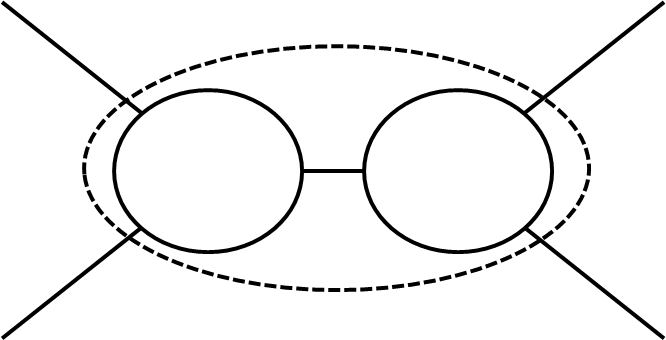
\includegraphics[width=0.5\textwidth]{img/RandomizedReductionContraction}
\caption{Contracted 3-degree vertices act like a 4-degree vertex}
\label{figure:RandomizedReductionContraction}

\end{figure}



\subsubsection{Reduction for 3-edge-colored graph}
For the purpose of showing lower bounds on the local lemma in the LOCAL model, it is sufficient to show it for 3-edge-colored 3-regular graphs.  Using the observation above, we note that each of the three edge colors form a perfect matching.


\begin{algorithm}[H]\label{Graph reduction algorithm_colored}\small
	\caption{\small Graph reduction algorithm($DependancyGraph$)}
	\begin{itemize}
		\item Take $M$ to be the perfect matching which is the set of edges of color $1$.
		\item Contract vertices sharing edges $(u,v) \in M$. (contraction may create double edges)
		\item Denote $G'$ as the multi-graph  created by this process
	\end{itemize}
\end{algorithm}

We note that each vertex $v$ in $G'$ has degree exactly $d(v)=4$, and that Any distributed algorithm on $G'$ can be simulated by $G$ with constant overhead, by having a contracted node in $G'$ be simulated by the two nodes in $G$ that form it.  

\begin{lemma}
	Given a sinkless orientation on $G'$, a sinkless orientation can be found on the network $G$ in constant time.
\end{lemma}
\begin{proof}
	Consider a partial orientation on $G$ induced by  the uncontracted edges in $G$ (which are the edges in $G'$), and giving them the same orientation. If $G'$ is sinklessly oriented, then each matched pair has an edge leaving one of its vertices. Direct each of the contracted edges so that both matched vertices touching each edge are satisfied. This is possible since if a contracted vertex $w_{uv}$ isn't a sink in $G'$, then it has an outgoing edge, meaning that in $G$ either $u$ or $v$ have an outgoing edge, and therefore isn't a sink. Assume w.l.o.g that $v$ isn't a sink, then directing the edge $\{v,u\}$ towards $u$ makes it so both $v$ and $u$ are not sinks
\end{proof}

All that remains is to obtain a sinkless orientation for multi-graphs of degree $4$. This can be obtained using the distributed LLL similar to the $4$-regular case. By choosing the edge direction at random, the probability that a vertex is a sink is exactly $\frac{1}{2^4}$, on the other hand, each vertex has of at most $4$ distinct neighbors, therefore it has degree at most $4$ in the dependency graph. since $ep(d+1) = e\frac{5}{16} < 1$, we obtain a sinkless orientation via the use of the distributed local lemma, which concludes the reduction.


\subsubsection{Algorithm for general 3-regular graphs}

In the previous case, we used a perfect matching to reduce to the 4-regular case. a perfect matching is sufficient, but don't necessarily exist, or are hard to obtain in general $3$-regular graphs. In this subsection we show that a maximal matching is sufficient for the reduction. This is not needed for the lower bound on the Lovasz Local Lemma, but can be used as a tool to solve variants of the sinkless orientation, such as sinkless sourceless orientation. To find a maximal matching $M$, and contract matched vertices into a new 4-degree vertex (figure \ref{figure:RandomizedReductionContraction}). After that, the graph is almost a 4-regular graph, up to the unmatched isolated vertices. These will be forced by the reduction to act as an edge between two neighboring 4-degree vertices (figure \ref{figure:RandIsoVert}). 

\begin{figure}[h]
	\centering
	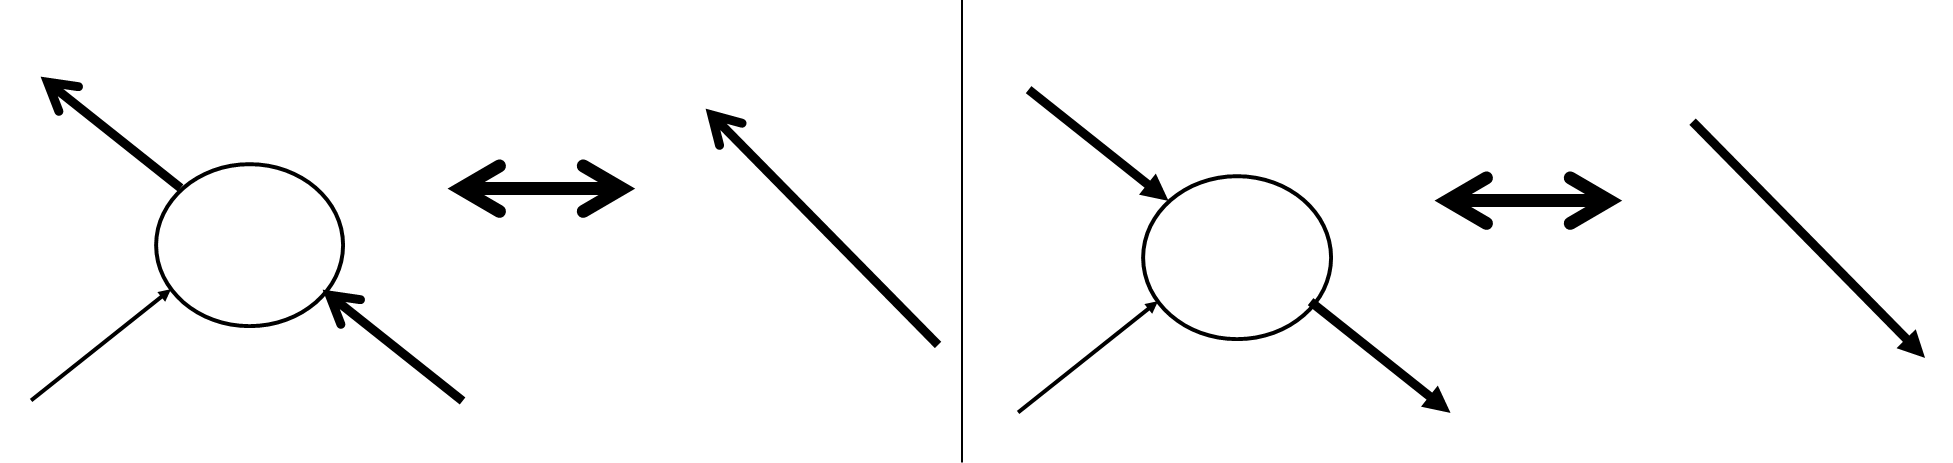
\includegraphics[width=1.0\textwidth]{img/RandomizedReductionIsolatedVertex}
	\caption{After fixing one of their edges inward, we can make isolated unmatched vertices acts as an edge between two matched neighboring vertices}
	\label{figure:RandIsoVert}
\end{figure}
\begin{algorithm}[H]\label{Graph reduction algorithm}\small
\caption{\small Graph reduction algorithm($DependancyGraph$,$M$)}
Denote the multi-graph created by this process $G'$:
\begin{itemize}
\item Contract vertices sharing edges $(u,v) \in M$. (contraction may create double edges)
\item For each isolated unmatched vertex $u$, replace two arbitrary edges $(u,v_1),(u,v_2)$ with an edge $(v_1,v_2)$, and remove the vertex and third edge
\end{itemize}
\end{algorithm}



\begin{lemma}
Given an orientation on $G'$ such that each $u \in \{v|d(v)=4\}$ is not a sink, a sinkless orientation can be found on the network $G$ in constant time.
\end{lemma}
\begin{proof}
\label{LLLThreeRegComplexLemma}
For each edge in $G'$ created by two edges of an isolated vertex $u$ in $G$, direct them both as directed by $G'$ as shown in figure \ref{figure:RandIsoVert}. Direct the third edge of an isolated vertex into the isolated vertex. The remaining non-matching edge in $G$ exist in $G'$ and direct them the way it is directed in $G'$. For isolated vertices, we note that no matter how we orient an edge in $G'$, it has an outgoing edge. Since it is a sinkless orientation in $G'$, then each matched pair has an edge leaving one of its vertices. Direct the edges in the matching $M$ so that both matched vertices are satisfied. This is possible since if a contracted vertex $w_{uv}$ isn't a sink in $G'$, then in $G$ either $u$ or $v$ isn't a sink.
\end{proof}

\begin{lemma}
Directing $G'$ to an orientation such that all 4-degree vertices are not a sink can be reduced to solving an LLL instance of the same size.
\end{lemma}
\begin{proof}
This is similar to the 4-regular case. Choose a random orientation for all edges in $G'$. In this case only 4-degree vertices sinks are considered bad events, and we note that the dependency graph has dependency $4$, and each two vertices in the dependency graph are at most of distance $2$ in the communication graph. Bad events as before have $Pr(A_v) \leq \frac{1}{16}$ as each of their edges are chosen uniformly and independently.  Since $ep(d+1) = e\cdot \frac{1}{16}\cdot 5 < 1$, it follows that the LLL algorithm converges after $O(log^2(d) \cdot \log{n}) = O(\log{n})$ rounds, meaning we get an orientation such that any $u \in \{v|d(v)=4\}$ isn't a sink. From Lemma \ref{LLLThreeRegComplexLemma} we can obtain a sinkless orientation on $G$ in constant time.
\end{proof}


\begin{algorithm}\label{ThreeRegularReduction}\small
\caption{\small ThreeRegularReduction($DependancyGraph$)}
\begin{itemize}
\item Obtain a MIS $M$ of $G$.
\item Calculate $G'$ using $M$
\item Run an LLL algorithm on the graph $G'$
\item Translate the directions into $G$ in the following manner:
\begin{itemize}
\item If $e \in G'$ is an edge in both $G$ and $G'$ direct it in the same manner as $G'$.
\item If $e \in G'$ was created by two edges of an isolated vertex, direct them the same way as the edge in $G'$ as shown in figure \ref{figure:RandIsoVert}.
\item If $e=(u,v)$ ia an edge in $M$, then direct it so that both $u$ and $v$ aren't sinks
\end{itemize}
\end{itemize}
\end{algorithm}

\begin{theorem}
 A 3-regular graph sinkless orientation instance can be reduced to a Distributed Lovasz Local Lemma instance in $O(log^*n)$ rounds.
\end{theorem}
\begin{proof}
Obtaining an MIS takes $O(\log^* n)$ rounds on bounded degree graphs, reduction to $G'$ takes $O(1)$ rounds, And by using the LLL algorithm on $G'$ the instance can be solved.
\end{proof}
\begin{corollary}
Sinkless orientation on 3-regular graphs can be solved in $O(\log n)$ rounds.
\end{corollary}

\subsection{Conclusion}
We've studied the sinkless orientation problem, shown a deterministic algorithm, and shown a reduction to the Lovasz Local Lemma in regular graphs, overcoming a difficulty in the case $d=3$, where the LLL criteria is too weak for it. We note that using the distributed algorithmic Lovasz Local Lemma we can solve similar problems to the sinkless orientation, such as sinkless sourceless orientations, even if at first they don't seem to meet the criteria of the LLL using the tools in the final subsection. This is done iteratively by constructing a new multi-graph by gaining a maximal matching, amplifying the success probability of each bad event, until the LLL criteria is met.

\section{An $O(\log{n})$ Deterministic Algorithm For Sinkless Orientation in the CONGEST model}
 A natural question regarding Sinkless orientation is if it can be done efficiently while restricting the edge bandwidth in each round to be $O(\log{n})$ (i.e the CONGEST model). For a randomized protocol, the LLL algorithm of \cite{KMPHH14} gives us an immediate positive answer. This is due to the fact that their algorithm consists of finding a maximal independent set of bad event vertices in the dependency graph and re-sampling them, but the bad events defined in section \ref{sec:rand_lovasz} clearly form an independent set, as if $v$ is a sink, then all of its neighbors in $G$ must not be sinks, as they have an outgoing edge to $v$, and so by lemma \ref{lem:rand_sink_dep_graph} part (2) the claim follows. For a deterministic algorithm, naively implementing the algorithm in section \ref{AlgSection} would not work, as each vertex learns its $\log{n}$ neighborhood, and therefore has a very high message length. in the following section we give an efficient algorithm for sinkless orientation in a restricted bandwidth model to the deterministic case as well.

In this algorithm, having vertices attempt to orient a path connected to a cycle plays a key role as well, but we can't have each vertex learning such a path and cycle, as it might be too expensive to do in parallel. 

\begin{definition}
	$v$ is a dominating vertex if it has the maximum id in its $2\log{n}$ neighborhood
\end{definition}
Each dominating vertex can safely perform a BFS on its $\log{n}$ neighborhood without interference from other dominating vertices. It is not clear how such a vertex learns the path and cycle in a restricted bandwidth setting. For this we define cycle witnesses
\begin{definition}
	Denote a vertex $u$ a witness cycle from a vertex $v$ with regards to a BFS protocol originating from $v$ if it has received at least two incoming messages during the BFS.
\end{definition}
We note that these messages must be received in two different edges.The key idea of the algorithm is as follows: each dominating vertex $v$ orients a path and a cycle. It does so by performing a BFS on its $\log{n}$ neighborhood, finding a cycle witness $u$. By definition a cycle witness has two edges in which it has received a BFS message. By considering two tokens - a red token and a blue token, each starting at $u$. $u$ sends one token through each such edge, and then the token backwards traversal through the BFS up to the root $v$. We note that the edges on which a token was traveresed form a path connected to a cycle (See figure). Oriented correctly, this yields a directed path starting from $v$, connected to an oriented cycle that contains $u$. The process above satisfies the dominating vertices, and the part of their $\log{n}$ neighborhood participating in the path and cycle defined above (denoted active nodes in the algorithm). The rest of the vertices are not satisfied by this process, but as will be shown later, is sufficient if each non-active (passive) vertex picks the edge from its edges that is closest to the largest id in its $2\log{n}$ neighborhood ($passiveParent$) and orient it outwards.

\begin{figure}[h]
	\centering
	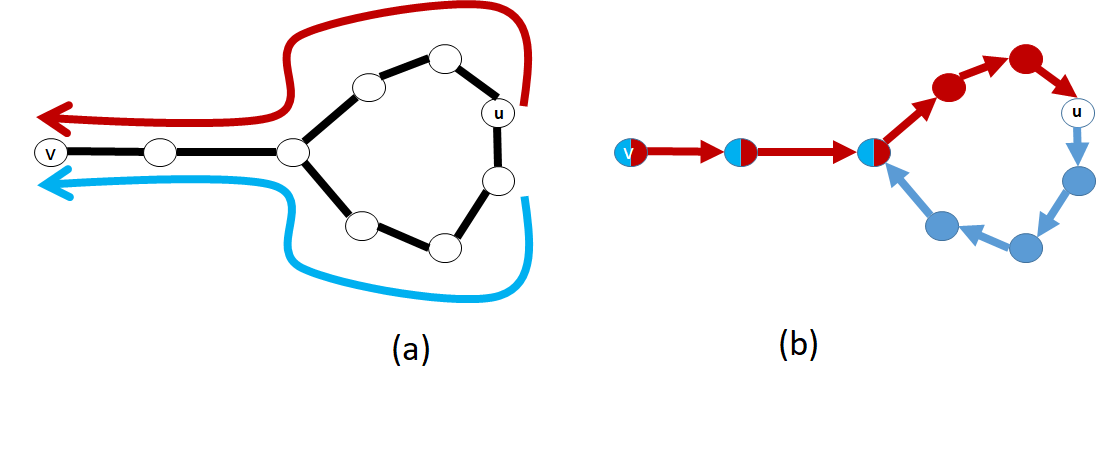
\includegraphics[width=0.8\textwidth]{img/CongestFigure.png}
	\caption{\\(a) The path of the tokens from the chosen witness $w$ to its dominating vertex $v$ \\(b)The orientation each edge receives in this process.If it seen only blue - towards parent,if it seen red - towards child}
\end{figure}



\begin{algorithm}[H]\label{alg:sinkless_congest}\small
	\caption{\small SinklessCongest($G$)}
	\begin{itemize}
		\item Using a priority BFS for $2\log{n}$ rounds from all vertices, each vertex checks if it is a dominating vertex, and if not it saves two pointers - $passiveRoot,passiveParent$ as the maximum id encountered and the edge in which it entered the earliest (breaking ties by ids of parents).
		\item Each dominating vertex starts a BFS for $\log(n)$ rounds. Note that as two dominating vertices have a distance of at least $2\log{n}$, the two BFS originating from them are disjoint
		\item All cycle witnesses of a vertex $v$ from the BFS send their id through their parent vertex in the BFS up to their root by priority BFS for $\log(n)$ steps. 
		\item If a dominating vertex $v$ receives a cycle witness, it chooses the cycle witness with the largest id and sends it to its $\log{n}$ neighborhood
		\item The chosen witness of $v$ chooses two incoming edges of the BFS, sends a red token through one, and a blue token through the second. These tokens traverse back through the parent edges until reaching back to $v$. 
		\item Through each edge that the red token traversed, direct the parent edge towards the child. If the blue token passes to the parent edge, and the red token did not, direct it towards the parent. If a vertex encounters any token in this phase, it marks itself as active, otherwise it marks itself passive
		\item Each passive vertex directs its $passiveParent$ edge outwards  
		\item Direct any undirected edge into the larger id 
	\end{itemize}
\end{algorithm}

\begin{lemma}
	Each dominating vertex receives a cycle witness during the algorithm.
\end{lemma}
\begin{proof}
	As two dominating vertices have distance at least $2\log{n}$, the BFS is uninterrupted by other dominating vertices.By Lemma \ref{lem:near_cycle}, each vertex has a cycle of length $\log{n}$ in its $\log{n}$ neighborhood. Therefore in a BFS of length $\log{n}$, at least one vertex from that cycle receives two messages.
\end{proof}

\begin{lemma}
	\label{lem:active_good}
	Edges oriented by active nodes of a dominating vertex $v$ before the end of the algorithm form a directed path connected to a directed cycle, where each edge is between two active vertices.
\end{lemma}
\begin{proof}
	Let $u$ be the chosen witness of $v$. All such edges are oriented by the red and blue token traversal. As the red and blue tokens originate together from $u$, and they move at the first step into two different vertices, and both reach $v$, there must be a vertex $w$ in which they both "re-meet" (in the sense that they both go through $w$). Furthermore, as they both traverse on parents of the BFS, once they "re-meet", the path traversed from $w$ to $v$ is traversed from both. The union of the two (disjoint) paths traversed up to $w$ is $u$ by both tokens form a cycle, and the path from $w$ to $v$ forms a path. The way the algorithm orients them forms a directed path, connected to a directed cycle. Clearly all nodes with edges oriented this way in the algorithm have a token traversing through them, therefore all edges are between two active vertices.  
\end{proof}
\begin{lemma}
	Edges orientations  of the algorithm are well defined.
\end{lemma}
\begin{proof}
	Consider the edges oriented before the last step. By Lemma \ref{lem:active_good}, all edges oriented by active nodes of a dominating vertex $v$ form a path connected to a cycle and are well defined. A passive vertex only orients the edge $passiveParent$. If its $passiveParent$ is between two passive nodes, the edge orientation is well defined unless the two vertices have the same edge pointer of $passiveParent$.  They have to be different, as if the $id$ of $passiveRoot$ is the same at both vertices, then the earliest entry time of the message to their $passiveParent$ edge differs by one, by definition of BFS, indicating that $passiveParent$ is not the same edge. In the case that $passiveRoot$ is different in these two vertices, which clearly indicates that $passiveParent$ is different. If the edge is between a passive and active node it is well defined as by Lemma \ref{lem:active_good} all edges oriented by active nodes are between two active nodes. Clearly all remaining unoriented edges in the last step are oriented in a consistent manner.
\end{proof}
\begin{corollary}
	\label{lem:congest_is_sinkless}
	The oriented edges of $G$ form a sinkless orientation.
\end{corollary}
\begin{proof}
	As each passive vertex has an outgoing edge to its $passiveParent$, and each active vertex has an outgoing edge as it participates in a directed path that connects into a directed cycle, all vertices have an outgoing edge.
\end{proof}

\begin{theorem}
	SinklessCongest terminates after $O(\log{n})$ rounds and  the orientation obtained is a sinkless orientation.  
\end{theorem}
\begin{proof}
	The round complexity is clearly $O(\log{n})$, as the time complexity of each step is bounded by at most $2\log{n}$ rounds, and by Corollary \ref{lem:congest_is_sinkless} the orientation obtained is a sinkless orientation.   
\end{proof}